\chapter{SUR/FACE} 
\label{sec:baydoor}
\lstset{style=6502Style}

Take a moment to consider how we might compose the surface of our dreadnoughts without
specifying each tile painstakingly for each row and column. One approach would be
to instead define smaller structures and piece those together to form a greater whole.

Consider the example below, a structure on the forward section of the 'Gold' dreadnought
in Level 6. Spend a little time relating the definition on the right hand side with the
end result on the left. 

\begin{minipage}[c]{0.43\linewidth}
	\vspace{-0.2cm}
	\begin{figure}[H]
		\centering
		\begin{adjustbox}{width=4.7cm,center}
			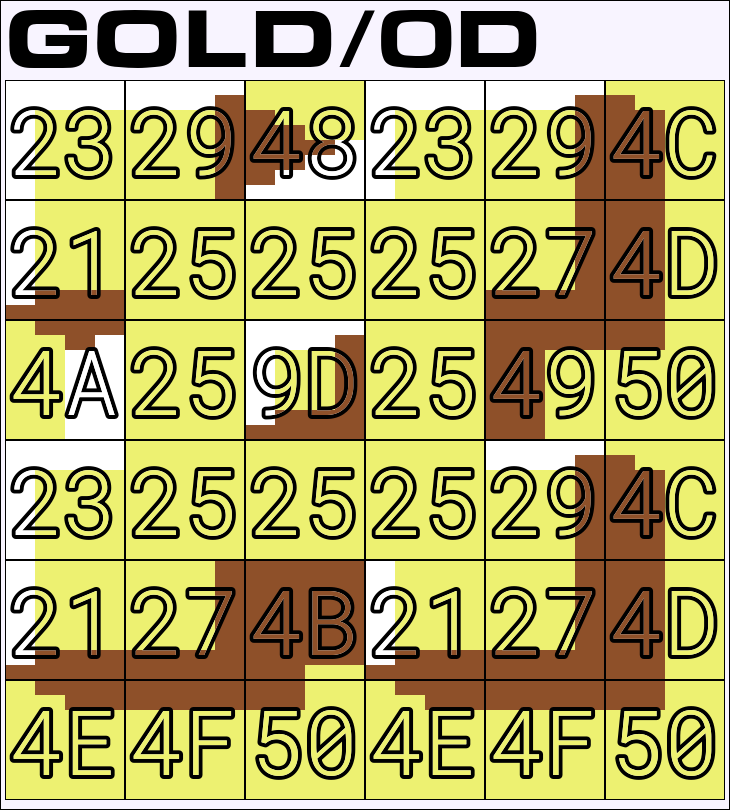
\includegraphics{src/surface_structure_diagrams/6_0D.png}%
		\end{adjustbox}
	\end{figure}
\end{minipage}
\begin{minipage}[c]{0.58\linewidth}
	\begin{lstlisting}[basicstyle=\footnotesize\ttfamily]
; Structure $0D
.BYTE $06   ; Number of vertical strips.
.BYTE $06   ; Strip 1 Length
.BYTE $4E,$21,$23,$4A,$21,$23 ; Strip 1
.BYTE $06   ; Strip 2: Length 
.BYTE $4F,$27,$25,$25,$25,$29 ; Strip 2
.BYTE $06   ; Strip 3: Length
.BYTE $50,$4B,$25,$9D,$25,$48 ; Strip 3
.BYTE $06   ; Strip 4: Length
.BYTE $4E,$21,$25,$25,$25,$23 ; Strip 4
.BYTE $06   ; Strip 5: Length
.BYTE $4F,$27,$29,$49,$27,$29 ; Strip 5
.BYTE $06   ; Strip 6: Length
.BYTE $50,$4D,$4C,$50,$4D,$4C ; Strip 6
\end{lstlisting}
\end{minipage}

Notice how we specify 6 vertical strips from left to right, designating the tiles to use for each strip
working from the bottom up. Try to pair the tile values in each array with their corresponding
positions in the diagram. Hopefully you can see how it works.

If we can define structures in this way, and give each one an index (such as \icode{\$0D} in this
example), then we have an inuitive way of constructing our dreadnought levels from building blocks.

\textit{Uridium} takes exactly this approach but splits it into two passes. We will cover the first pass
here, and the second pass in the following chapter. Our first pass is to create a sort of undercoat
for the level, a layer of sections of equal height that form the base of the structure. 

For Level 6 (\icode{Gold}) we can define this base layer with a list of numbers, each one an index
referencing one of the prefabricated sections on the opposite page.
\begin{lstlisting}
level6DreadnoughtData
  .BYTE $20,$20,$20,$20,$05,$04,$20,$20,$20,$20,$05,$04,$7A,$7B,$7B,$7B
  .BYTE $02,$5C,$06,$06,$06,$5C,$04,$7A,$7B,$7B,$7B,$02,$07,$20,$20,$20
  .BYTE $20,$0E,$0F,$0F,$0F,$02,$5C,$04,$0E,$0F,$0F,$0F,$02,$5C,$04,$0E
  .BYTE $0F,$0F,$0F,$20,$20,$20,$20,$05,$81,$84,$84,$84,$84,$84,$84,$5C
  .BYTE $5C,$82,$85,$85,$85,$85,$85,$85,$5C,$5C,$5C,$5C,$5C,$07,$0C,$08
  .BYTE $08,$08,$08,$08,$08,$08,$08,$05,$5C,$5C,$5C,$5C,$09,$0A,$0A,$0A
  .BYTE $0A,$0A,$0A,$0A,$0A,$0A,$0A,$67,$5C,$09,$0A,$0A,$0A,$0A,$0A,$0A
  .BYTE $0A,$0A,$0A,$0B,$20,$20,$20,$20,$20,$20,$20,$20,$20,$20,$20,$05
  .BYTE $07,$20,$20,$20,$20,$0C,$08,$08,$08,$08,$08,$20,$20,$20,$20,$05
  .BYTE $5C,$06,$06,$06,$06,$06,$06,$5C,$5C,$5C,$5C,$5C,$5C,$5C,$5C,$5C
  .BYTE $04,$00
\end{lstlisting}

Our layer starts with the empty space of 4 stripes of section \icode{\$20}, followed by \icode{\$05}, \icode{\$04}
and so on. Using the first 13 bytes from the array above we can see how the bow of the dreadnought is built up from left to right.

\begin{figure}[H]
    \begin{adjustbox}{width=13.2cm,left}
      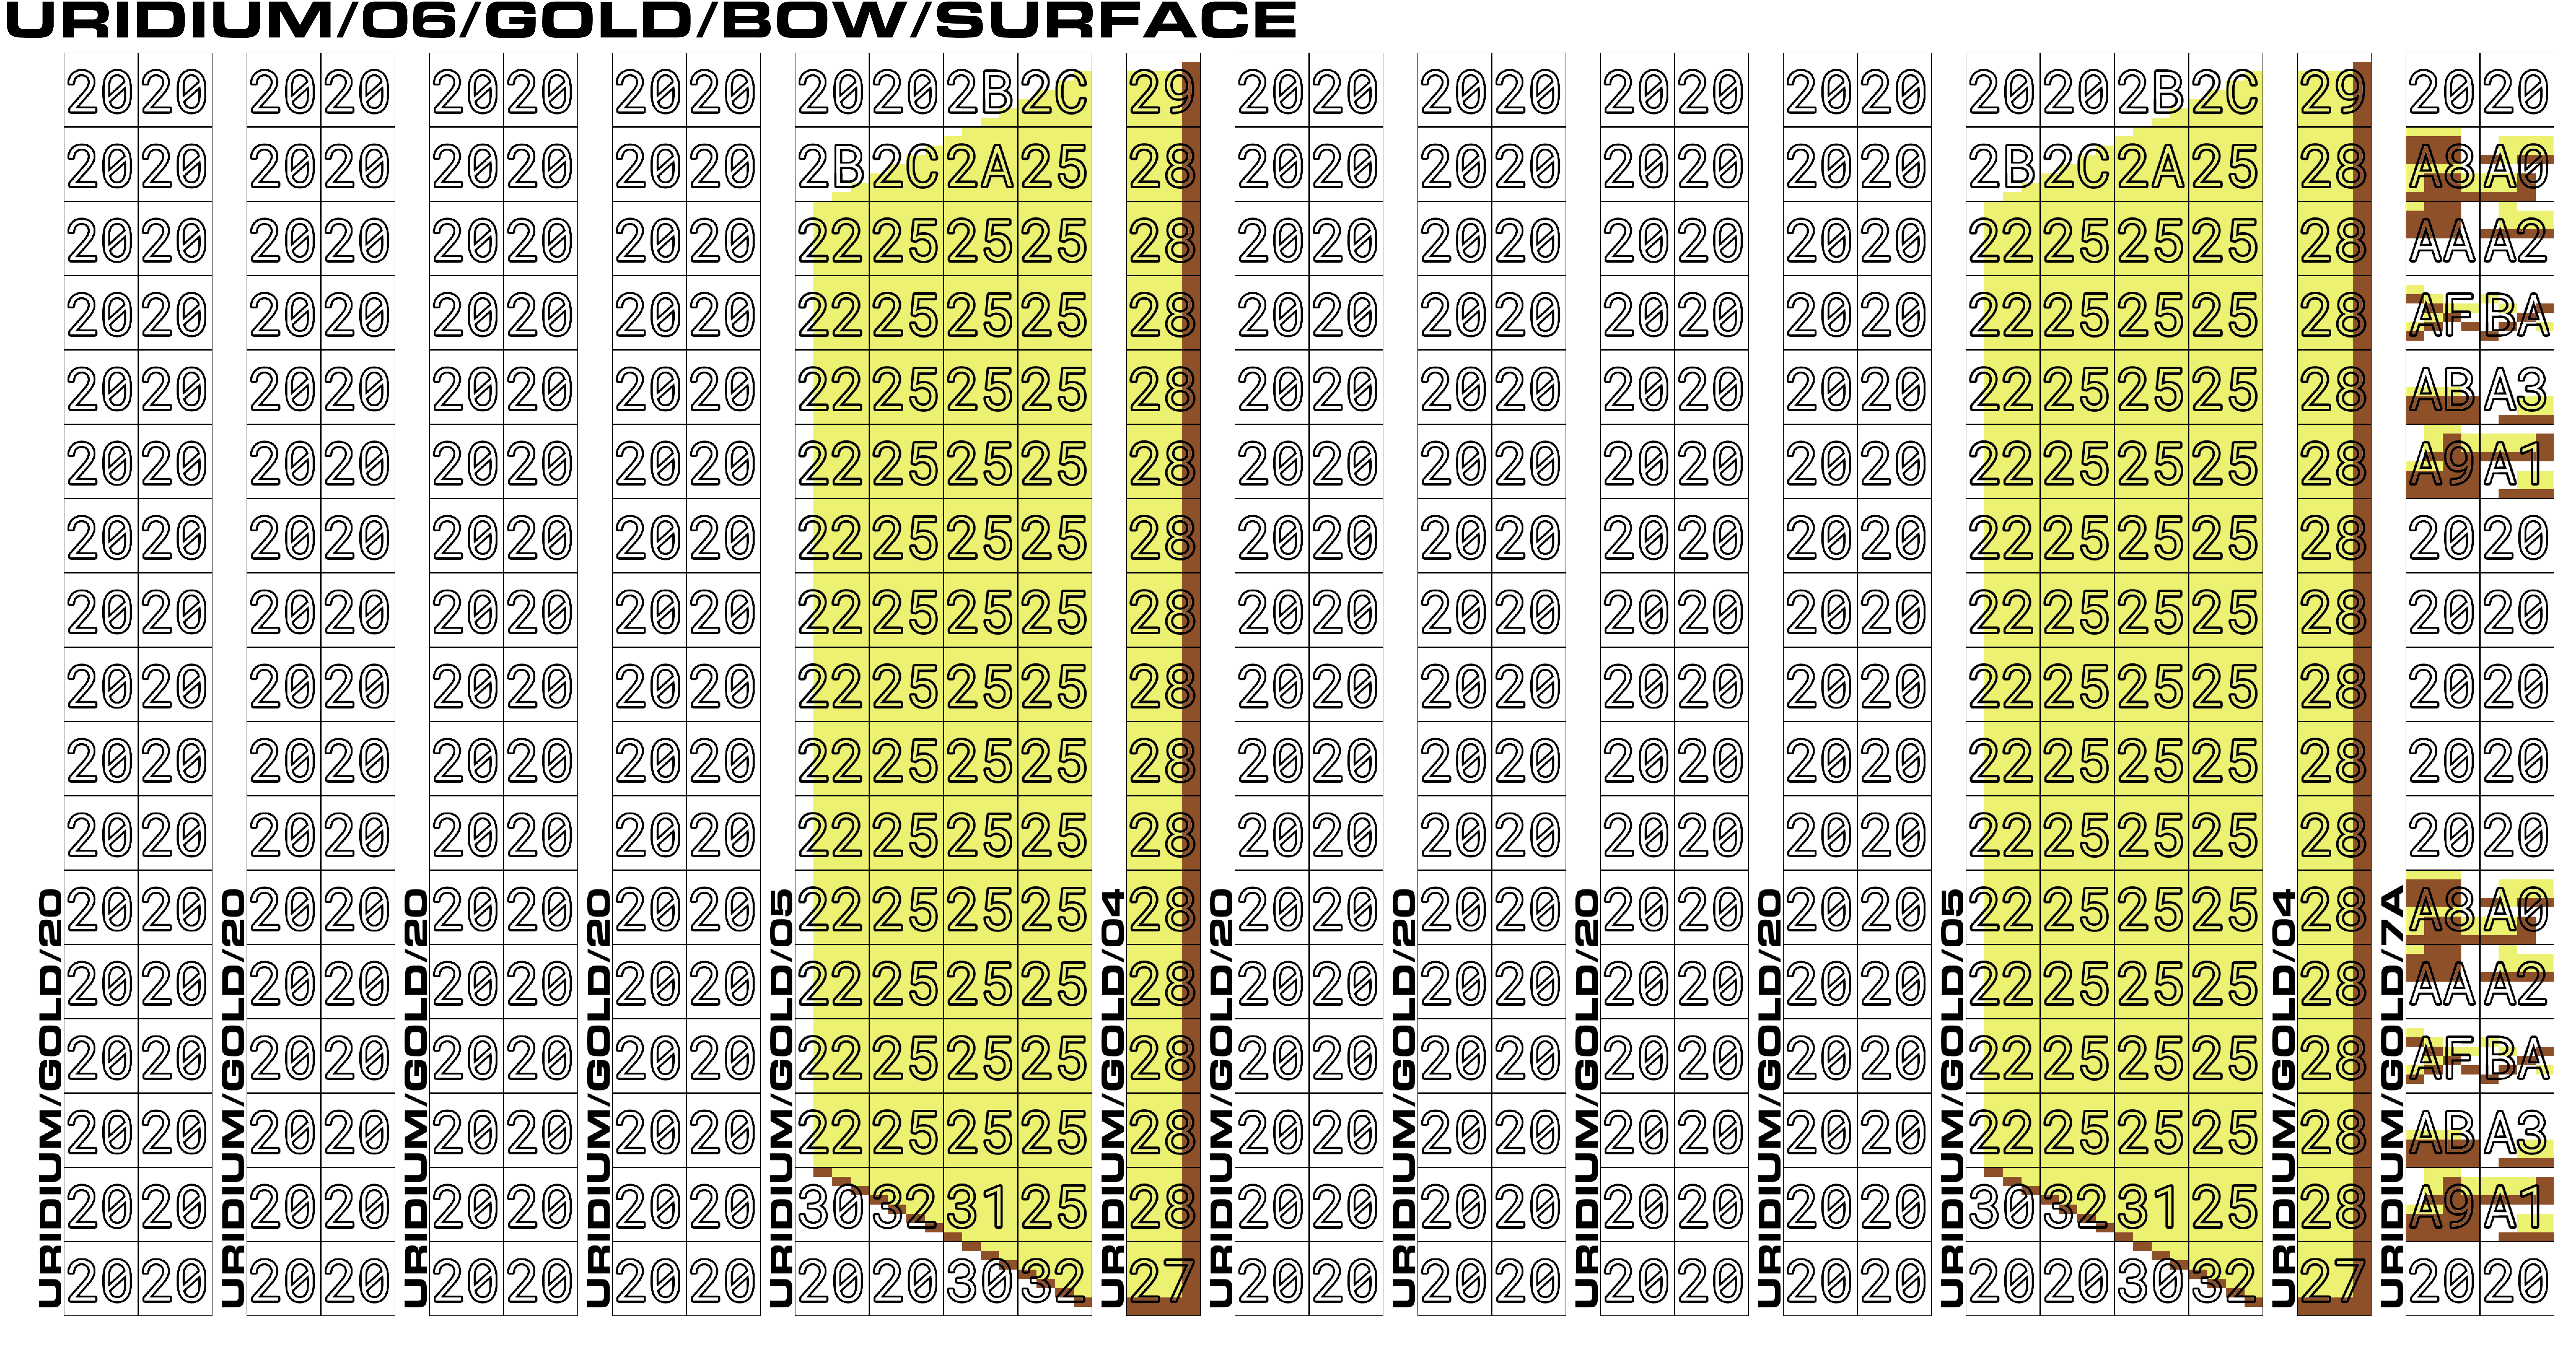
\includegraphics{src/surface_diagrams_with_sections/6_1.png}%
    \end{adjustbox}
\end{figure}
\vspace{-0.4cm}

\clearpage

\raisebox{-0.1\totalheight}{
\includegraphics[height=9.2cm]{src/surface_section_diagrams/6_20_large_text.png}}
\raisebox{-0.1\totalheight}{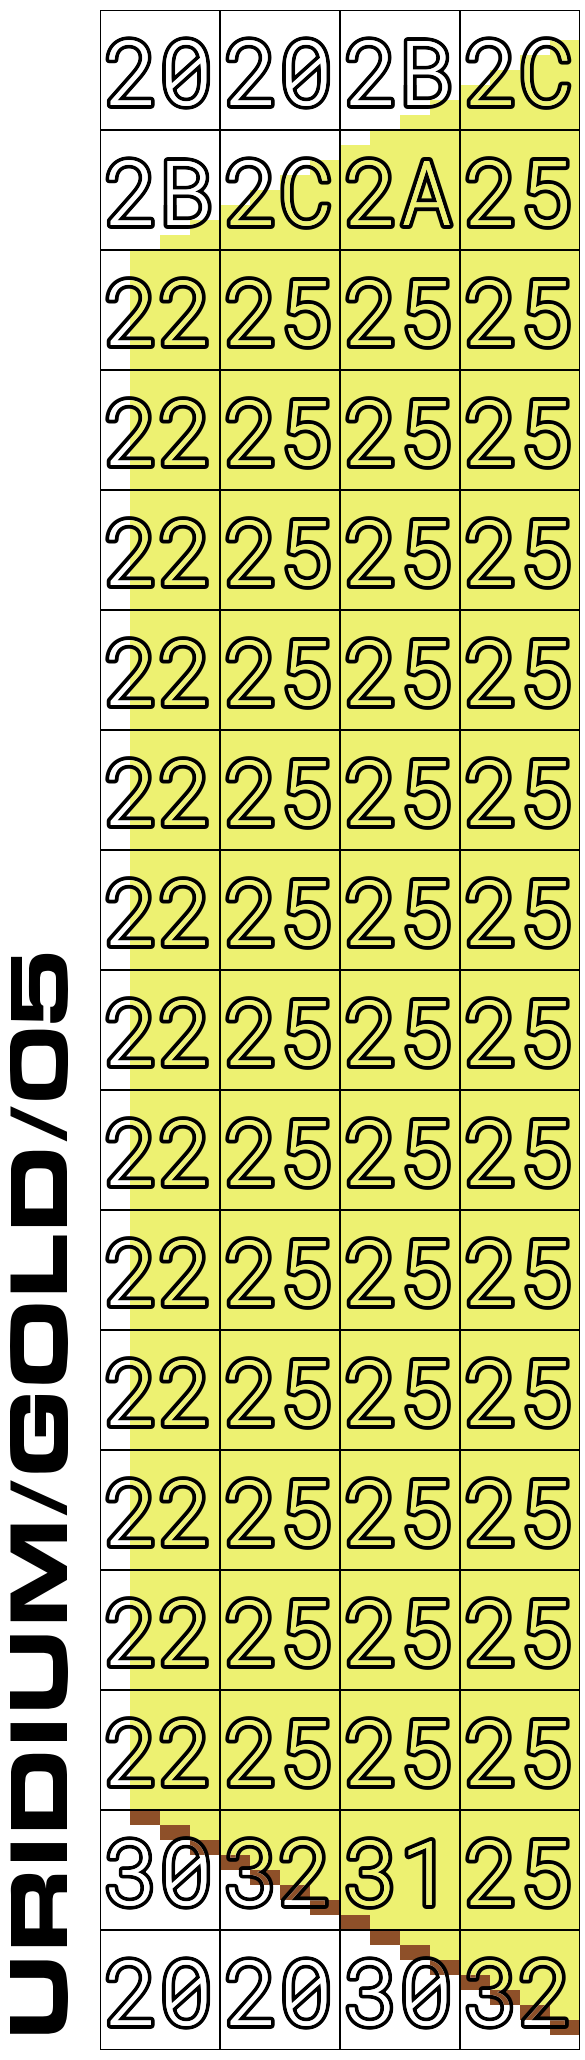
\includegraphics[height=9.2cm]{src/surface_section_diagrams/6_05_large_text.png}}
\raisebox{-0.1\totalheight}{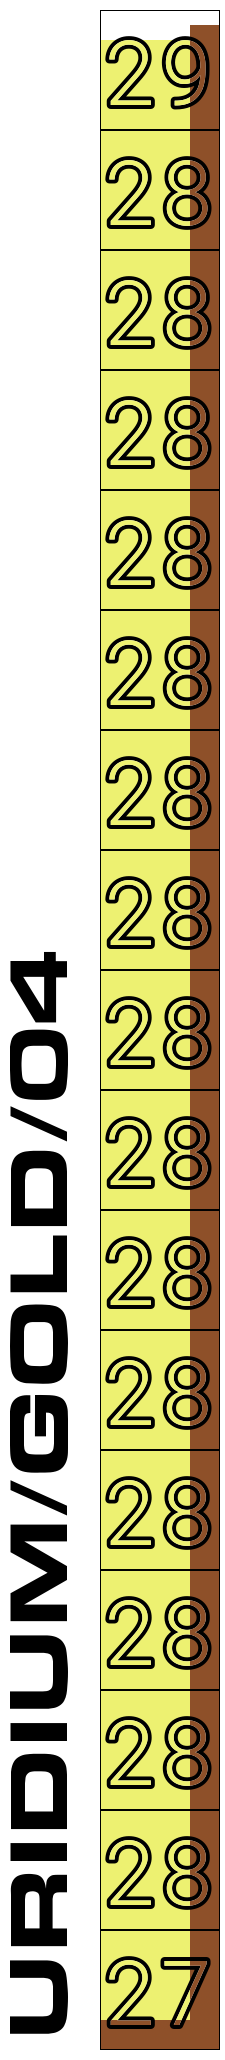
\includegraphics[height=9.2cm]{src/surface_section_diagrams/6_04_large_text.png}}
\raisebox{-0.1\totalheight}{
\includegraphics[height=9.2cm]{src/surface_section_diagrams/6_7A_large_text.png}}
\raisebox{-0.1\totalheight}{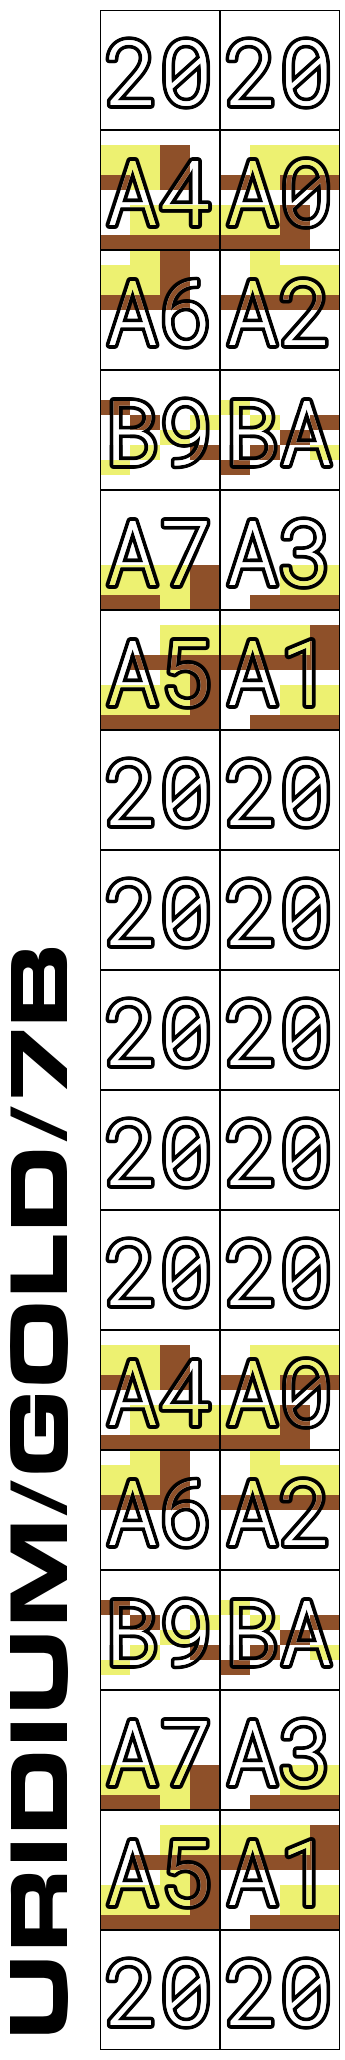
\includegraphics[height=9.2cm]{src/surface_section_diagrams/6_7B_large_text.png}}
\raisebox{-0.1\totalheight}{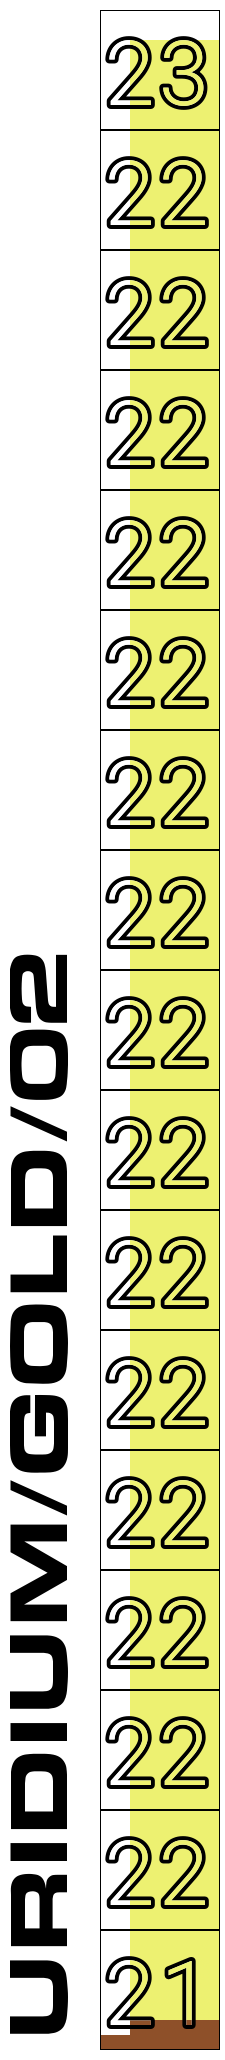
\includegraphics[height=9.2cm]{src/surface_section_diagrams/6_02_large_text.png}}
\raisebox{-0.1\totalheight}{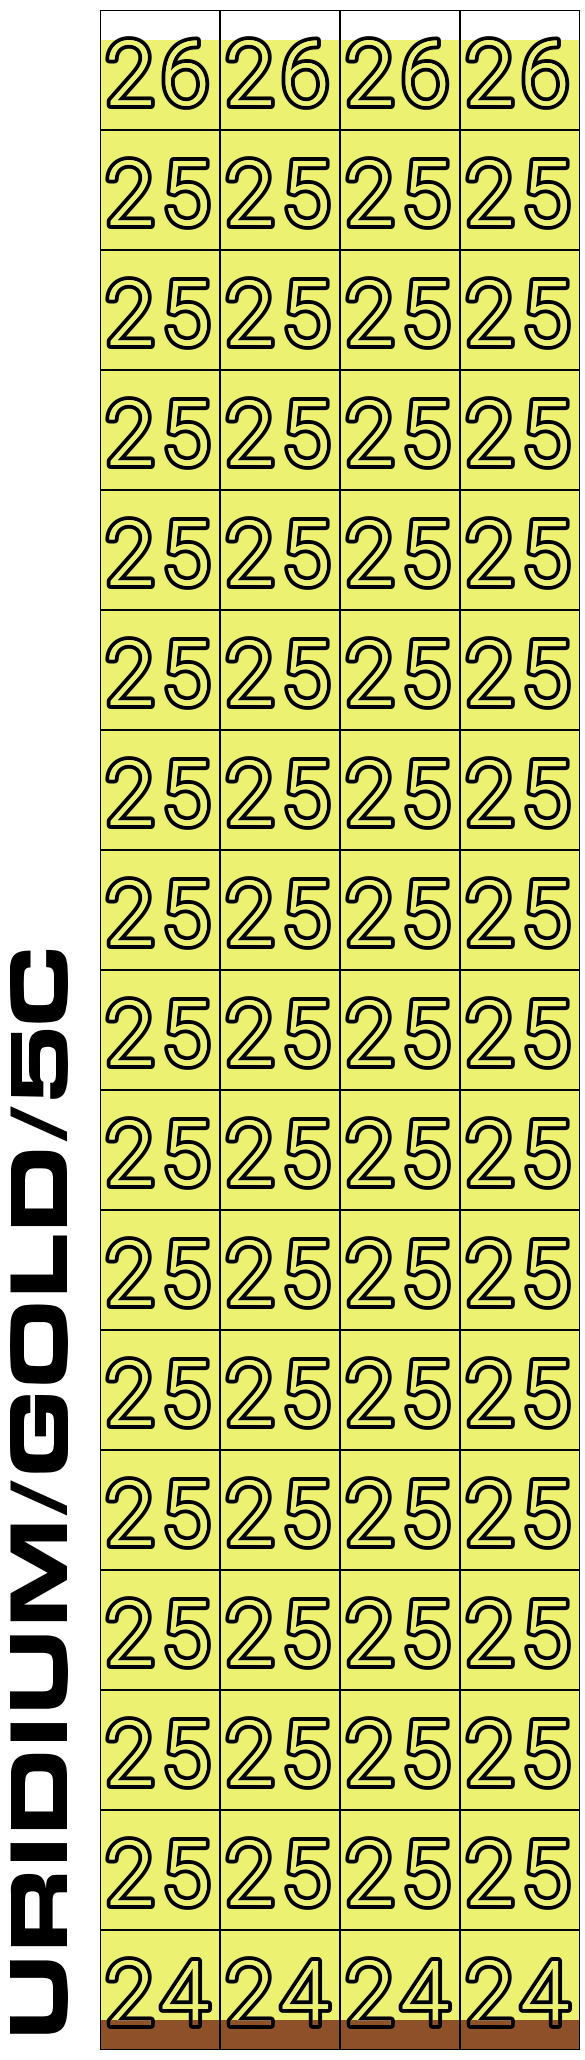
\includegraphics[height=9.2cm]{src/surface_section_diagrams/6_5C_large_text.png}}
\raisebox{-0.1\totalheight}{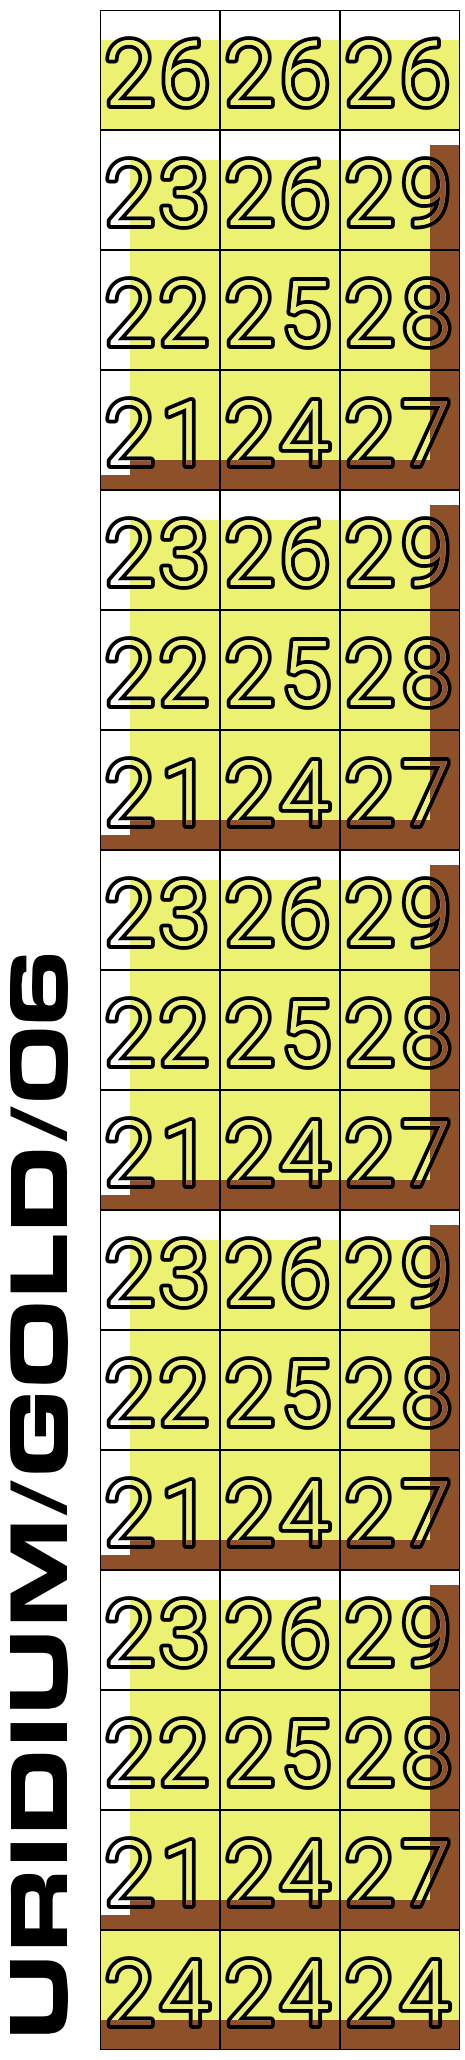
\includegraphics[height=9.2cm]{src/surface_section_diagrams/6_06_large_text.png}}
\raisebox{-0.1\totalheight}{
\includegraphics[height=9.2cm]{src/surface_section_diagrams/6_0E_large_text.png}}
\raisebox{-0.1\totalheight}{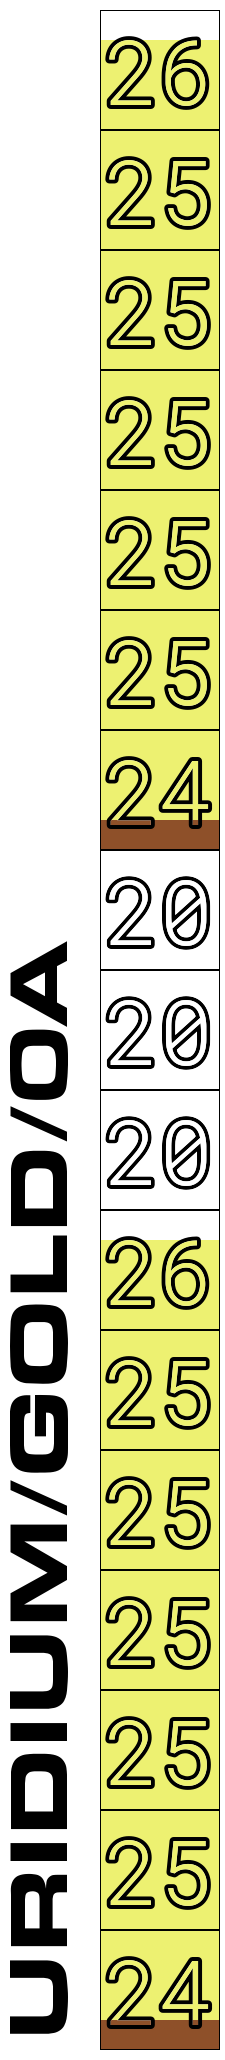
\includegraphics[height=9.2cm]{src/surface_section_diagrams/6_0A_large_text.png}}
\raisebox{-0.1\totalheight}{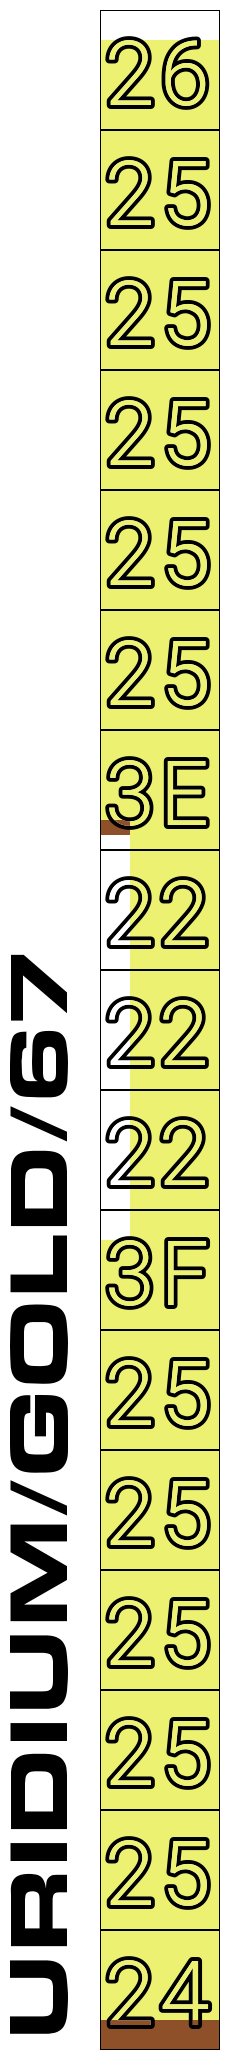
\includegraphics[height=9.2cm]{src/surface_section_diagrams/6_67_large_text.png}}
\raisebox{-0.1\totalheight}{
\includegraphics[height=9.2cm]{src/surface_section_diagrams/6_08_large_text.png}}
\raisebox{-0.1\totalheight}{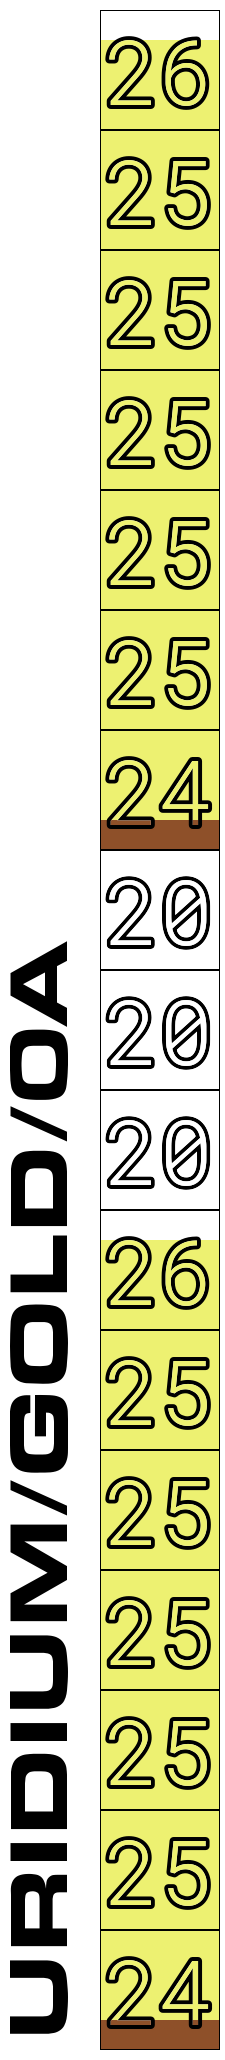
\includegraphics[height=9.2cm]{src/surface_section_diagrams/6_0A_large_text.png}}
\raisebox{-0.1\totalheight}{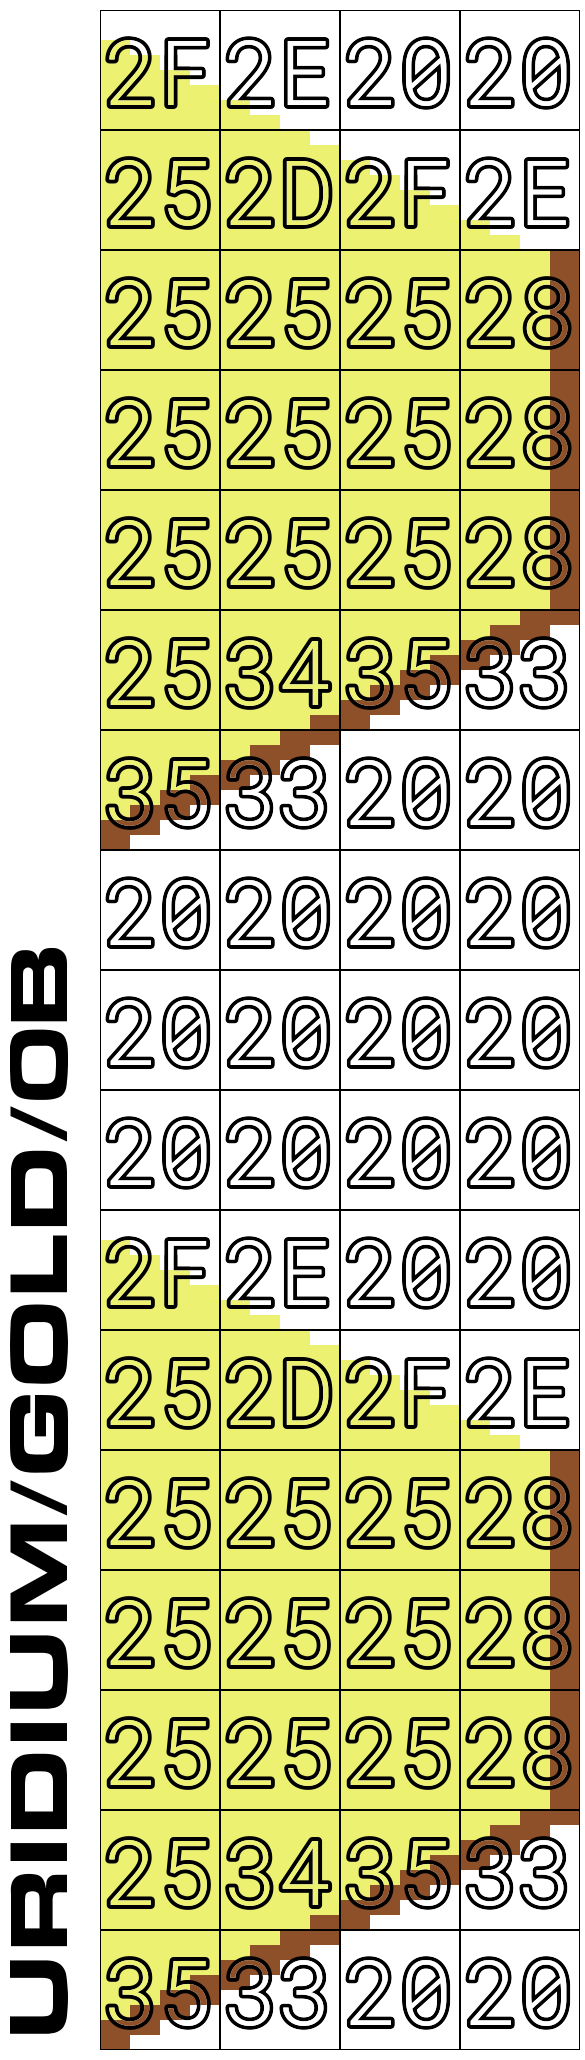
\includegraphics[height=9.2cm]{src/surface_section_diagrams/6_0B_large_text.png}}
\raisebox{-0.1\totalheight}{
\includegraphics[height=9.2cm]{src/surface_section_diagrams/6_0C_large_text.png}}
\raisebox{-0.1\totalheight}{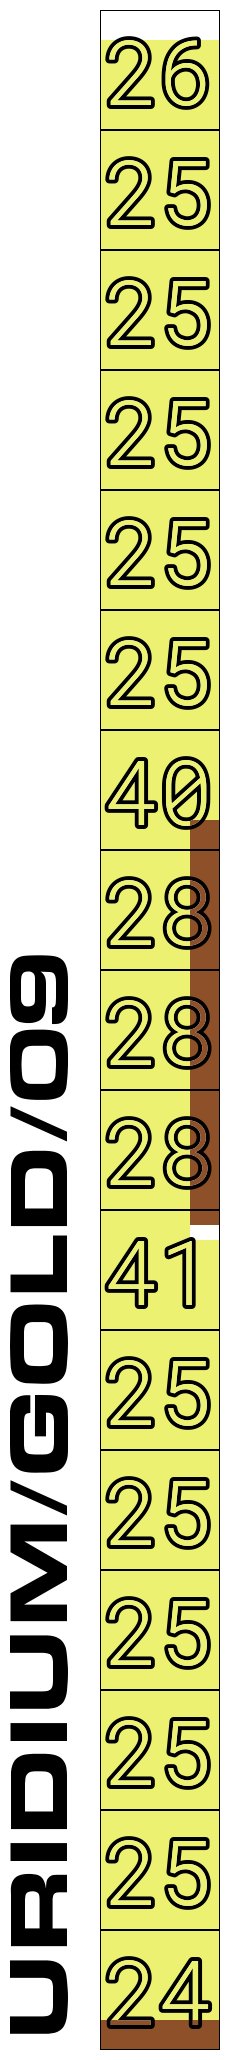
\includegraphics[height=9.2cm]{src/surface_section_diagrams/6_09_large_text.png}}
\raisebox{-0.1\totalheight}{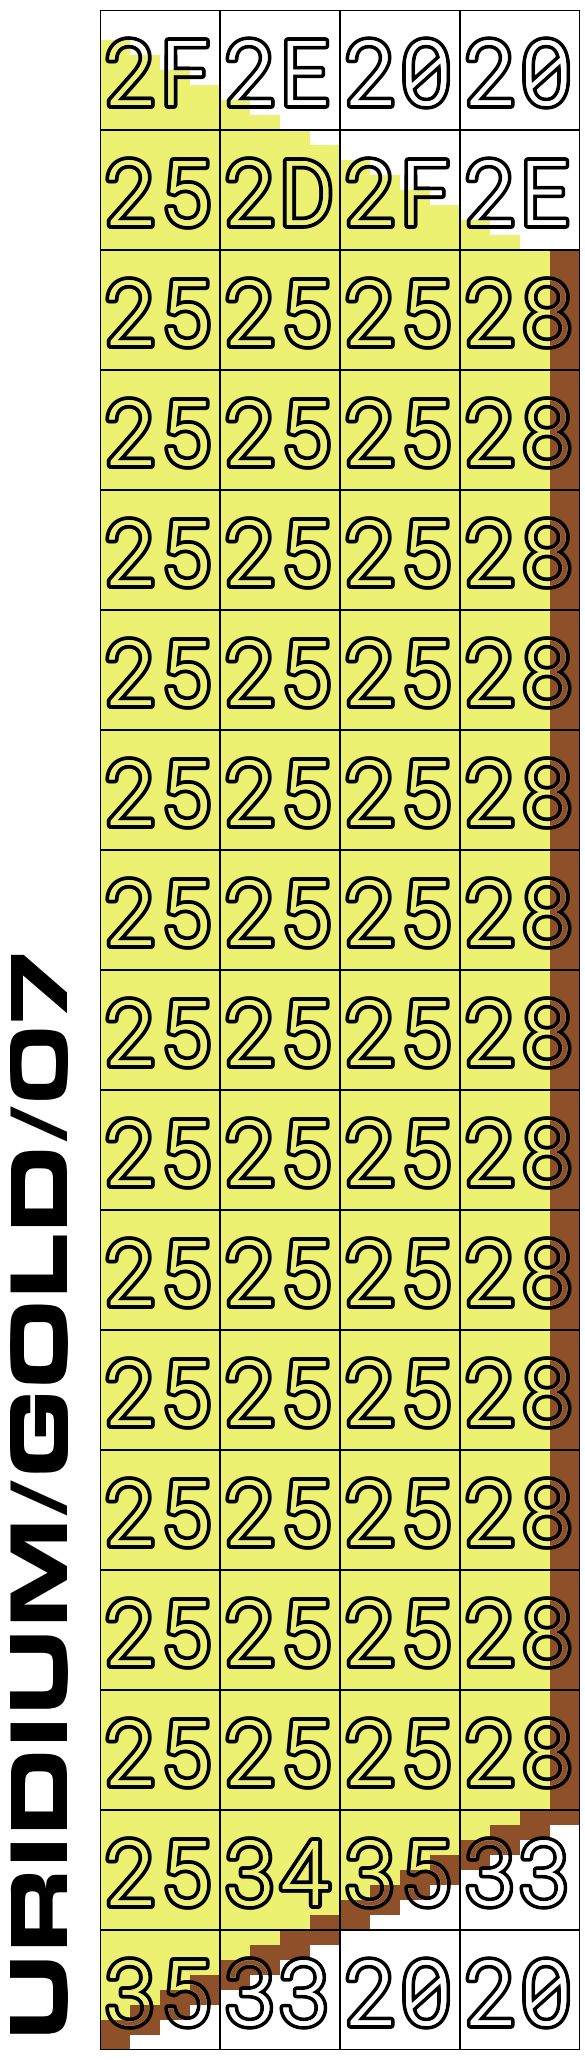
\includegraphics[height=9.2cm]{src/surface_section_diagrams/6_07_large_text.png}}

\clearpage
If you'd like to try to follow in detail how this process was implemented in practice, you can take
some time to read the routine on the opposite page. Imagine the \icode{DrawSurfaceSections} outer loop
reading in each byte from \icode{level6Dreadnought\-Data}
above, looking up the section data that a byte (for example, \icode{\$05}) references, and then observe how the \icode{DrawSectionStrip} inner
loop processes a piece of section data like \icode{\$05} below to draw it on to the screen.
\footnote{In the extract opposite, to keep the code legible and fit the routine on a single page I have removed some of the verbose book-keeping that 6502 assembly code requires. For example \icode{CLC} instructions which are sometimes necessary before an addition operation are left out.}.

\begin{minipage}[c]{0.23\linewidth}
	\vspace{-0.2cm}
	\begin{figure}[H]
		\centering
		\begin{adjustbox}{height=6.5cm,center}
			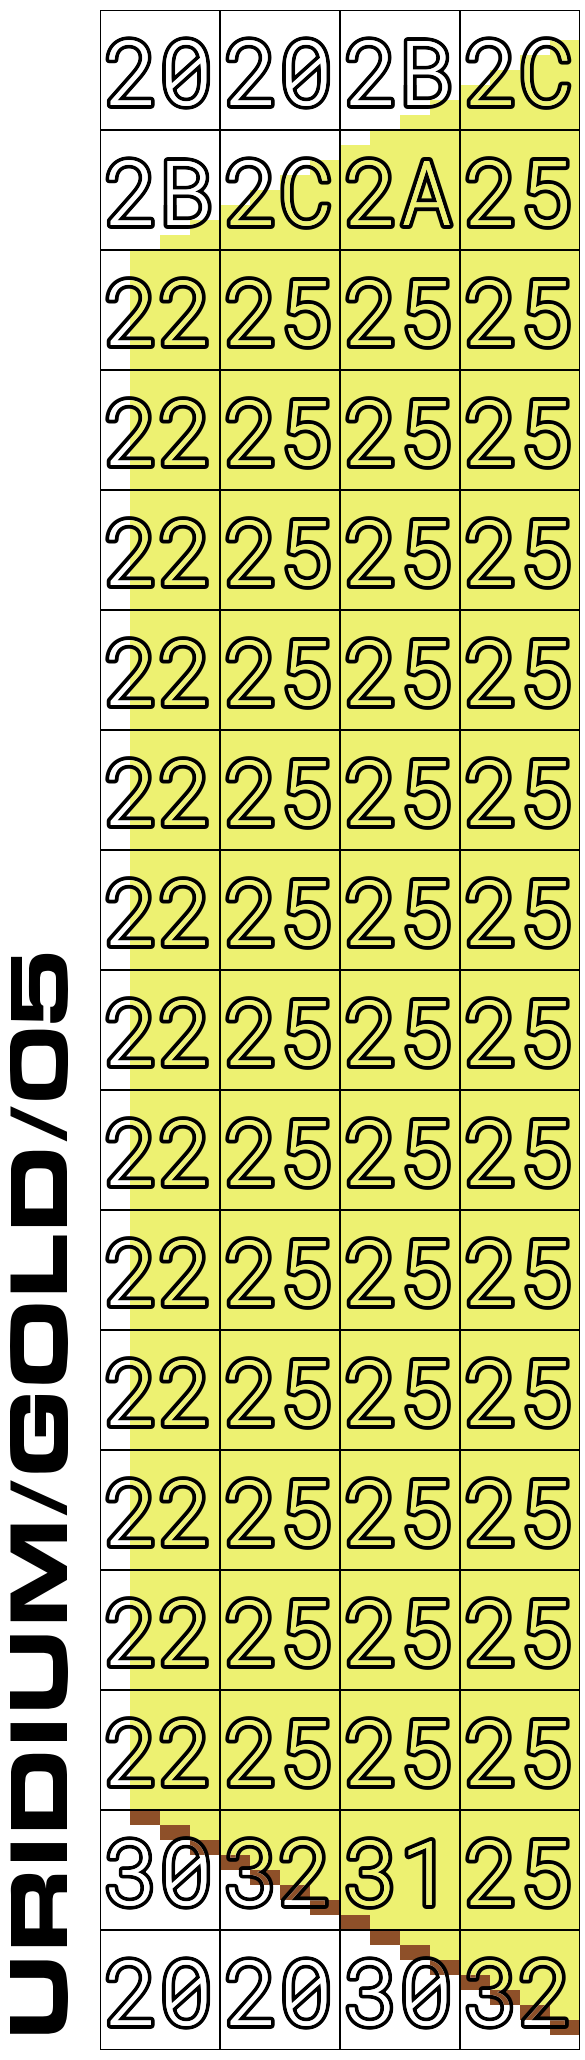
\includegraphics{src/surface_section_diagrams/6_05_large_text.png}%
		\end{adjustbox}
	\end{figure}
\end{minipage}
\begin{minipage}[c]{0.78\linewidth}
\begin{lstlisting}[basicstyle=\footnotesize\ttfamily]
; Section $05
.BYTE $04 ; Number of vertical strips (4)
.BYTE $10 ; Strip 1: Length 16
 ; Strip 1: Character Set Tiles
.BYTE $20,$30,$22,$22,$22,$22,$22,$22
.BYTE $22,$22,$22,$22,$22,$22,$22,$2B
.BYTE $10 ; Strip 2: Length 16 
 ; Strip 2: Character Set Tiles
.BYTE $20,$32,$25,$25,$25,$25,$25,$25
.BYTE $25,$25,$25,$25,$25,$25,$25,$2C
.BYTE $11 ; Strip 3: Length 17
 ; Strip 3: Character Set Tiles
.BYTE $30,$31,$25,$25,$25,$25,$25,$25
.BYTE $25,$25,$25,$25,$25,$25,$25,$2A,$2B
 ; Strip 4: Character Set Tiles
.BYTE $11 ; Strip 4: Length 17
.BYTE $32,$25,$25,$25,$25,$25,$25,$25
.BYTE $25,$25,$25,$25,$25,$25,$25,$25,$2C 
\end{lstlisting}
\end{minipage}


Notice that each strip is drawn from the bottom up. And that we fill in any blank spaces to the top of
the screen that are left undefined by the strip (such as in strips 1 and 2 above).

Once \icode{DrawSurfaceSections} has run, and processed the entire array of bytes in \icode{level6\-Dreadnought\-Data},
we get the following result:
\begin{figure}[H]
    \begin{adjustbox}{width=14cm,center}
      
\includegraphics{src/surfaces_raw_surface_only/6.png}%
    \end{adjustbox}
\end{figure}
\vspace{-0.4cm}
You can now see what we meant about a 'first pass'. The main surface elements are present but a quick
visual comparison shows all of the features in the final product, as well as some more detailed sections, are missing:

\begin{figure}[H]
    \begin{adjustbox}{width=14cm,center}
      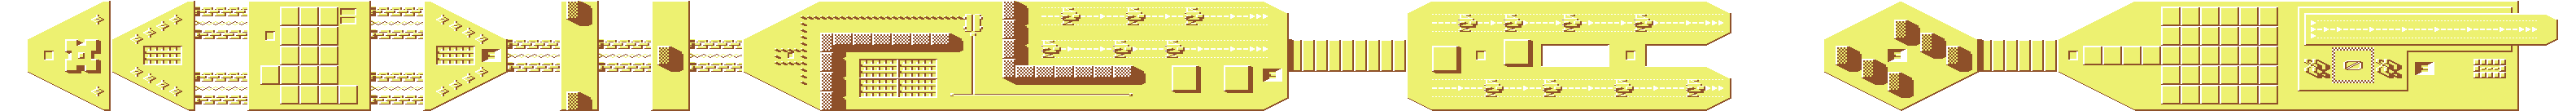
\includegraphics{src/surfaces_raw/6.png}%
    \end{adjustbox}
\end{figure}
\vspace{-0.4cm}

\clearpage

\begin{lstlisting}[basicstyle=\scriptsize\ttfamily]
DrawSurfaceSections   
  LDY #$00                     ; Set Y to zero.
  LDA (dreadnoughtDataLoPtr),Y ; Read a byte from dreadnought data to A.
  BEQ FinishedSurfaceLoop      ; If it's zero, we've reached the end.
  TAX                          ; Store the byte in X.
  ; Use the byte to point to the section data.
  LDA surfaceStructureDataHiPtrArray,X  ; Get the High Byte of the section.
  STA sectionDataHiPtr         ; Store it.
  LDA surfaceStructureDataLoPtrArray,X  ; Get the Low Byte of the section.
  STA sectionDataLoPtr         ; Store it.
  ; Move our pointer to next byte in dreadnought data, for next time around.
  LDA dreadnoughtDataLoPtr     ; Get the current pointer.
  ADC #$01                     ; Increment it.
  STA dreadnoughtDataLoPtr     ; Store it.

  ; The start of each section data contains the number of strips in the section.
GetNumberOfStrips   
  LDA (sectionDataLoPtr),Y     ; Read number of strips in to 'A'.
  INY                          ; Move our pointer to the next byte in the data.
  STA numberOfStrips           ; Store the number of strips.

  ; Draw each strip of the section.
DrawSectionStrip   
  LDA (sectionDataLoPtr),Y     ; Read in the length of the strip.
  INY                          ; Move index to next position.
  TAX                          ; Store the length in X.
ReadSectionBytes   
  LDA (sectionDataLoPtr),Y   ; Get a charset value from the section and store in A.
  INY                        ; Increment our pointer to the data.
  STY stashedYValue          ; Stash it.
  LDY #$00                   ; Use Y as a pointer to the surface. 
  STA (levelSurfaceLoPtr),Y  ; Write the charset value to the surface.
  LDY stashedYValue          ; Restore Y.
  DEC levelSurfaceHiPtr      ; Move up to the next position in the strip (512 bytes) ..
  DEC levelSurfaceHiPtr      ; .. by decrementing the high pointer twice.
  DEX                        ; Decrement our counter.
  BNE ReadSectionBytes       ; Loop until the strip has been read in full.

  ; Fill any remaining vertical space left by the strip with blank spaces.
BlankSpacesLoop   
  LDA levelSurfaceHiPtr      ; Get our current vertical position.
  CMP #>topOfSurfaceData     ; If we have reached the top..
  BCC GoToNextStrip          ; .. then do the next strip in the section.
  ; Otherwise write a space to the current position.
  LDY #$00                   ; Use Y to point to current position in surface.
  LDA #SPACE                 ; Put a space character tile in 'A'.
  STA (levelSurfaceLoPtr),Y  ; Write it to the surface.
  DEC levelSurfaceHiPtr      ; Move up to the next position in the strip (512 bytes) ..
  DEC levelSurfaceHiPtr      ; .. by decrementing the high pointer twice.
  JMP BlankSpacesLoop        ; Loop until we reach top of strip.

  ; Do the next strip and/or the next section until we're done.
GoToNextStrip   
  LDA levelSurfaceLoPtr      ; Get position of current strip on dreadnought.
  ADC #$01                   ; Increment by one in order to draw ..
  STA levelSurfaceLoPtr      ; .. the next strip in the next position to the right.
  LDA levelSurfaceHiPtr      ; Get the 'end' of the dreadnought.
  CMP #>endOfSurfaceData     ; Have we reached it yet?
  BCS DrawPlacedStructures   ; If so, we've finished drawing the surface section.
  DEC numberOfStrips         ; Otherwise, do the next strip in the section.
  BNE DrawSectionStrip       ; Keep looping until all strips in the section are done.

  BEQ DrawSurfaceSections    ; Keep looping until all sections are done.
\end{lstlisting}
\clearpage

We can observe this same incompleteness in the base layer in other levels.

\begin{figure}[H]
    \begin{adjustbox}{width=14cm,center}
      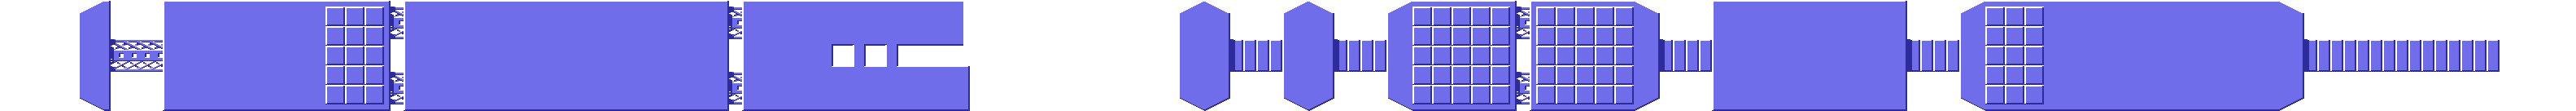
\includegraphics{src/surfaces_raw_surface_only/14.png}%
    \end{adjustbox}
\end{figure}
\vspace{-0.6cm}
\begin{figure}[H]
    \begin{adjustbox}{width=14cm,center}
      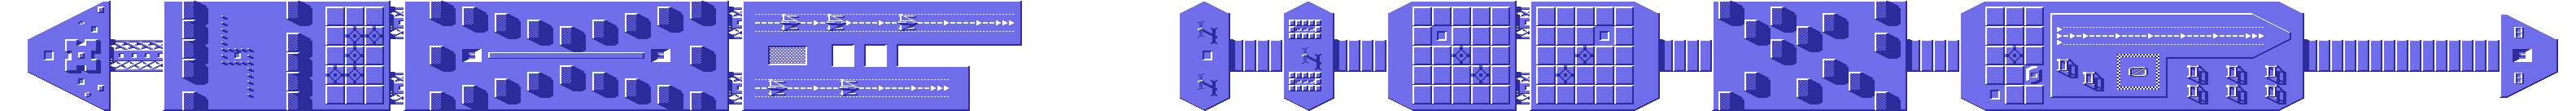
\includegraphics{src/surfaces_raw/14.png}%
    \end{adjustbox}
\end{figure}

\begin{figure}[H]
    \begin{adjustbox}{width=14cm,center}
      
\includegraphics{src/surfaces_raw_surface_only/11.png}%
    \end{adjustbox}
\end{figure}
\vspace{-0.6cm}
\begin{figure}[H]
    \begin{adjustbox}{width=14cm,center}
      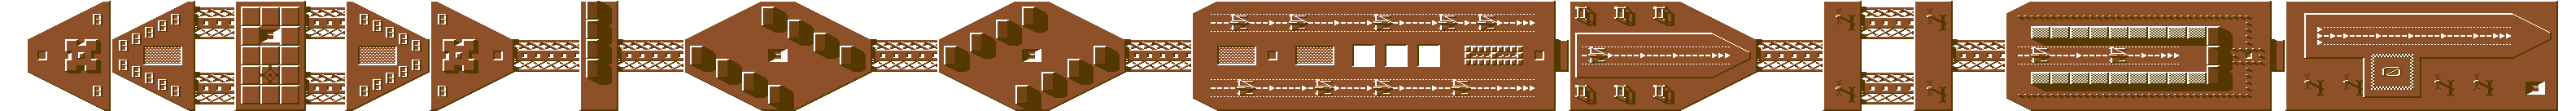
\includegraphics{src/surfaces_raw/11.png}%
    \end{adjustbox}
\end{figure}

But for some the first pass gives us something much closer to the finished product.

\begin{figure}[H]
    \begin{adjustbox}{width=14cm,center}
      
\includegraphics{src/surfaces_raw_surface_only/1.png}%
    \end{adjustbox}
\end{figure}
\vspace{-0.6cm}
\begin{figure}[H]
    \begin{adjustbox}{width=14cm,center}
      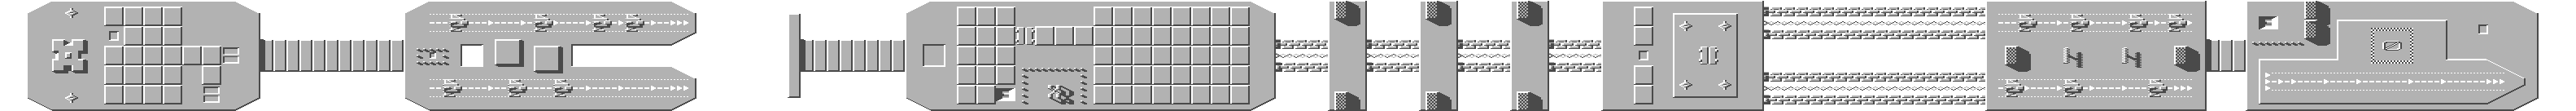
\includegraphics{src/surfaces_raw/1.png}%
    \end{adjustbox}
\end{figure}

\begin{figure}[H]
    \begin{adjustbox}{width=14cm,center}
      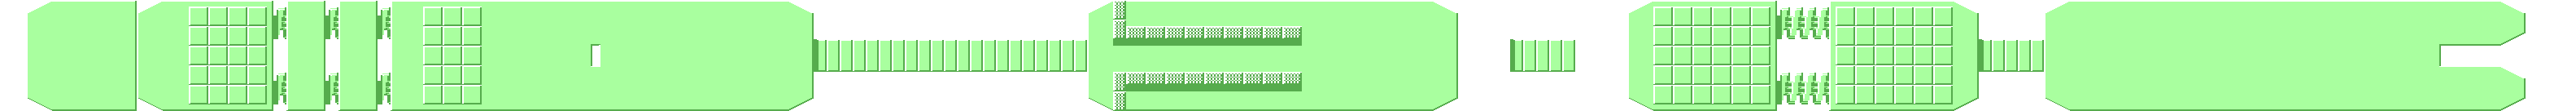
\includegraphics{src/surfaces_raw_surface_only/5.png}%
    \end{adjustbox}
\end{figure}
\vspace{-0.6cm}
\begin{figure}[H]
    \begin{adjustbox}{width=14cm,center}
      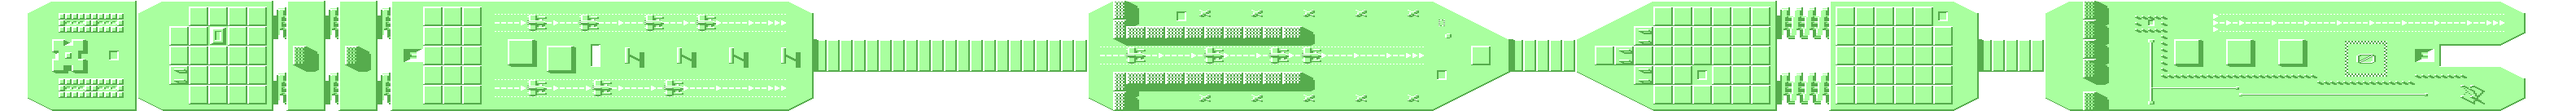
\includegraphics{src/surfaces_raw/5.png}%
    \end{adjustbox}
\end{figure}

\begin{figure}[H]
    \begin{adjustbox}{width=14cm,center}
      
\includegraphics{src/surfaces_raw_surface_only/2.png}%
    \end{adjustbox}
\end{figure}
\vspace{-0.6cm}
\begin{figure}[H]
    \begin{adjustbox}{width=14cm,center}
      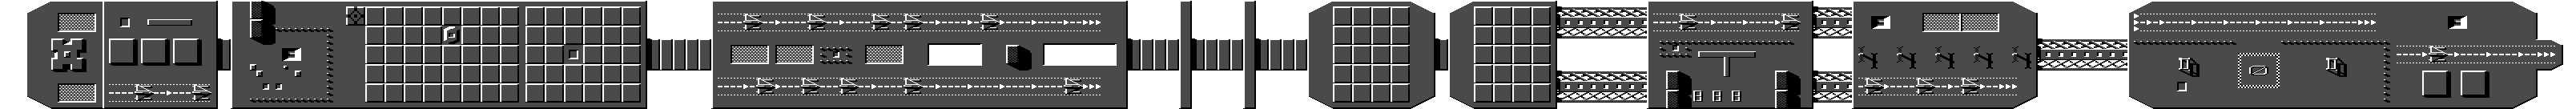
\includegraphics{src/surfaces_raw/2.png}%
    \end{adjustbox}
\end{figure}

We get a hint for why this might be when we compare the two phases of drawing Level 13 (\textit{Ergonite}):

\begin{figure}[H]
    \begin{adjustbox}{width=14cm,center}
      
\includegraphics{src/surfaces_raw_surface_only/13.png}%
    \end{adjustbox}
\end{figure}
\vspace{-0.6cm}
\begin{figure}[H]
    \begin{adjustbox}{width=14cm,center}
      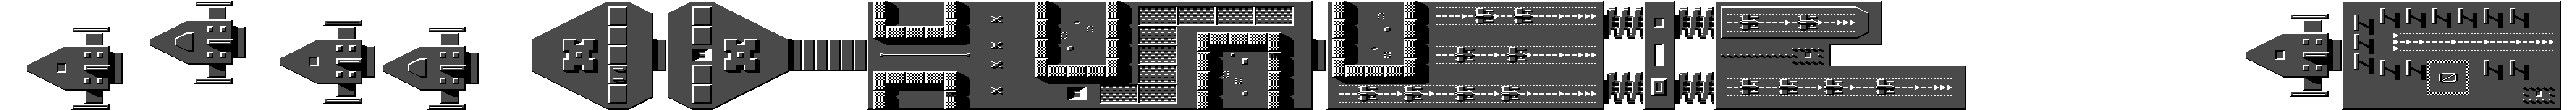
\includegraphics{src/surfaces_raw/13.png}%
    \end{adjustbox}
\end{figure}

Two of the ship-like structures are present in the first pass rather than being added in the second. Why would
this be? If we look attentively we can see the answer: all sections added in the first pass begin at the bottom
of the 'screen'. They have a fixed vertical position. So when we have a section that we will paint all the way to the bottom
we can include it in this first pass but if we want to place it elsewhere, further up the screen, we must
do so in the second pass.

Our next step is to find out more about this second pass and see how we go about the finishing phase required to create a completed dreadnought. How
we place the various detailed structures along the surface of the dreadnought to make it something worthy
of destruction.

